In the GLWE cryptosystem, modulus switching is a process of changing a ciphertext's modulo domain to a smaller (or larger) one, while ensuring that the ciphertext still decrypts to the same plaintext. For example, suppose we have the ciphertext $\textsf{LWE}_{S, \sigma}(\Delta m) \in \mathbb{Z}_q^{k+1}$. If we switch the ciphertext's modulo from $q \rightarrow q'$, then the ciphertext is converted into $\textsf{LWE}_{S, \sigma}\left(\Delta\dfrac{q'}{q} m\right) \in \mathbb{Z}_{q'}^{k+1}$. The ciphertext's all other components such as the noise ($e$) and public keys ($a_0, a_1, \cdots, a_{k-1}$, $b$) are scaled by $\dfrac{q'}{q}$, becoming $\left\lceil e\dfrac{q'}{q} \right\rfloor$, $\left(\left\lceil a_0\dfrac{q'}{q}\right\rfloor, \left\lceil a_1\dfrac{q'}{q}\right\rfloor, \cdots, \left\lceil a_{k-1}\dfrac{q'}{q}\right\rfloor, \left\lceil b\dfrac{q'}{q}\right\rfloor\right)$. To switch the modulo of an LWE ciphertext, we use the modulo rescaling technique learned from \autoref{sec:modulus-rescaling}. 
The same modulus switching technique can also be applied to RLWE ciphertexts. In this section, we will show how to switch (i.e., rescale) the modulo of LWE and RLWE ciphertexts and prove its correctness.  
%That is, after  LWE/RLWE ciphertexts, we will prove why they are still valid LWE/RLWE ciphertexts.


\subsection{LWE Modulus Switching}
\label{subsec:modulus-switch-lwe}

\textbf{- Reference:} 
\href{https://www.jeremykun.com/2022/07/16/modulus-switching-in-lwe/}{Modulus Switching in LWE}

$ $

Recall that the LWE cryptosystem (\autoref{subsec:lwe-enc}) comprises the following components:

\begin{itemize}
\item \textbf{\underline{Setup}:} $\Delta = \dfrac{q}{t}$, \text{ } $S = (s_0, s_1, \gap{$\cdots$} s_{k-1}) \xleftarrow{\$} \mathbb{Z}_2^{k}$

\item \textbf{\underline{Encryption Input}:} $m \in \mathbb{Z}_t$, \text{ } $A = (a_0, a_1, \text{ } \gap{$\cdots$} a_{k-1}) \xleftarrow{\$} \mathbb{Z}_q^{k}$, \text{ } $e \xleftarrow{\chi_\sigma} \mathbb{Z}_q$

$ $

\item \textbf{\underline{Encryption}:} $\textsf{LWE}_{S,\sigma}(\Delta  m) = (A, b) \in \mathbb{Z}_q^{k + 1}$ \text{ } (where $b = A \cdot S + \Delta  m + e \in \mathbb{Z}_q$)

$ $

\item \textbf{\underline{Decryption}:} $\textsf{LWE}^{-1}_{S,\sigma}(C) = b - A\cdot S = \Delta  m + e \text{ } \text{ } \in \mathbb{Z}_q$

\end{itemize}

$ $


In the LWE cryptosystem, modulus switching is a process of converting an original LWE ciphertext's modulo domain to a smaller modulo domain. This can be seen as scaling down all components, except for the plaintext $m$ and the secret key $S$, in the original LWE ciphertext to a smaller domain. This operation preserves the size and integrity of the original plaintext $m$, while the scaling factor $\Delta$ gets reduced to a smaller value $\hat{\Delta}$ and the noise $e$ to a smaller (reduced) noise $\hat{e}$ (note that noise alteration does not affect the original plaintext $m$, because the noise gets rounded away after decryption, anyway), and $A$ also gets scaled down to a smaller $\hat A$. Modulus switching is used for computational efficiency during TFHE's bootstrapping (which will be discussed in \autoref{subsec:tfhe-noise-bootstrapping}). Modulus switching is also used for implementing the ciphertext-to-ciphertext multiplication algorithm in BGV (\autoref{subsec:bfv-mult-cipher}) and CKKS (\autoref{subsec:ckks-mult-cipher}). 

The high-level idea of LWE modulus switch is to rescale the congruence relationship of the LWE scheme. LWE's homomorphic computation algorithms include the following: ciphertext-to-ciphertext addition, ciphertext-to-plaintext addition, ciphertext-to-plaintext multiplication, ciphertext-to-ciphertext multiplication. However, all congruence relationships used in these algorithms are essentially rewritten versions of the following single fundamental congruence relationship: $b = A\cdot S + \Delta m + e \bmod q$. Thus, modulus switch of an LWE ciphertext from $q \rightarrow q'$ is equivalent to rescaling the modulo of the above congruence relationship from $q \rightarrow q'$.

Based on this insight, the LWE cryptosystem's modulus switching from $q \rightarrow \hat{q}$ (where $q > \hat{q}$) is a process of converting the original LWE ciphertext $\textsf{LWE}_{S, \sigma}(\Delta m)$ as follows:

\begin{tcolorbox}[title={\textbf{\tboxlabel{\ref*{subsec:modulus-switch-lwe}} LWE Modulus Switching}}]

Given an LWE ciphertext $(A, b)$ where $b = A\cdot S + \Delta m + e \bmod q$ and $m \in \mathbb{Z}_t$, modulus switch of the ciphertext from $q$ to $\hat q$ is equivalent to updating $(A, b)$ to $(\hat A, \hat b)$ as follows:


$\hat{A} = (\hat{a}_0, \hat{a}_1, \gap{$\cdots$} \hat{a}_{k-1})$, where each $\hat{a}_i = \Big\lceil a\dfrac{\hat{q}}{q} \Big\rfloor \in \mathbb{Z}_{\hat{q}}$ \textcolor{red}{\# $\lceil \rfloor$ means rounding to the nearest integer}

 $\hat{b} = \Big\lceil b \dfrac{\hat{q}}{q} \Big\rfloor \in \mathbb{Z}_{\hat{q}}$

$\textsf{LWE}_{{S},\sigma}(\hat{\Delta}  m) = (\hat{a}_0, \hat{a}_1, \gap{$\cdots$}, \hat{b}) \in \mathbb{Z}_{\hat{q}}^{k + 1}$ 

$ $


The above update effectively changes $\hat e$ and $\hat \Delta$ as follows:

$\hat{e} = \Big\lceil e\dfrac{\hat{q}}{q} \Big\rfloor \in \mathbb{Z}_{\hat{q}}$, \text{ }

$\hat{\Delta} = \Delta\dfrac{\hat{q}}{q}$ \textcolor{red}{\# which should be an integer}

$ $


Meanwhile, $S$ and $m$ stay the same as before.

\end{tcolorbox}

$ $

 Note that in order for $(\hat{a}_0, \hat{a}_1, \gap{$\cdots$}, \hat{b}) \in \mathbb{Z}_{\hat{q}}^{k + 1}$ to be a valid LWE ciphertext of $\hat{\Delta}m$, we need to prove that the following relationship holds:

$\hat{b} = \sum\limits_{i=0}^{k-1}\hat{a}_i \cdot s_i + \hat{\Delta} m + \hat{e} \in \mathbb{Z}_{\hat{q}}$

$ $

%\textbf{\underline{Proof}}
\begin{myproof}
\begin{enumerate}
\item Note the following: 

$\hat{b} = \Big\lceil b \dfrac{\hat{q}}{q} \Big\rfloor = b\dfrac{\hat{q}}{q} + \epsilon_b$ (where $-0.5 < \epsilon_b < 0.5$, a rounding drift error)

$\hat{a_i} = \Big\lceil a_i \dfrac{\hat{q}}{q} \Big\rfloor = a_i\dfrac{\hat{q}}{q} + \epsilon_{a_i}$ (where $-0.5 < \epsilon_{a_i} < 0.5$)

$\hat{e} = \Big\lceil e \dfrac{\hat{q}}{q} \Big\rfloor = e\dfrac{\hat{q}}{q} + \epsilon_e$ (where $-0.5 < \epsilon_e < 0.5$)
\item Note the following: 

$b = \vec{a} \cdot \vec{s} + \Delta  m + e = \sum\limits_{i=0}^{k-1}(a_is_i) + \Delta m + e  \in \mathbb{Z}_q$

$b = \sum\limits_{i=0}^{k-1}(a_is_i) + \Delta m + e + H \cdot q$ (where modulo $q$ is replaced by adding $H \cdot q$, some multiple of $q$)

\item According to step 1 and 2:

$\hat{b} = b\dfrac{\hat{q}}{q} + \epsilon_b \in \mathbb{Z}_{\hat{q}}$

$= \left(\sum\limits_{i=0}^{k-1}(a_is_i) + \Delta m + e + H \cdot q\right) \cdot \dfrac{\hat{q}}{q}  + \epsilon_b$

$= \dfrac{\hat{q}}{q} \cdot \sum\limits_{i=0}^{k-1}(a_is_i) + \dfrac{\hat{q}}{q} \cdot \Delta m + \dfrac{\hat{q}}{q} \cdot e + \dfrac{\hat{q}}{q} \cdot H \cdot q + \epsilon_b$

$= \sum\limits_{i=0}^{k-1}\left(\dfrac{\hat{q}}{q} \cdot a_is_i\right) + \hat{\Delta} m + (\hat{e} - \epsilon_e) + \hat{q}\cdot H + \epsilon_b$

$= \sum\limits_{i=0}^{k-1}\left((\hat{a}_i - \epsilon_{a_i}) \cdot s_i\right) + \hat{\Delta} m + \hat{e} - \epsilon_e + \hat{q}\cdot H + \epsilon_b$

$= \sum\limits_{i=0}^{k-1}(\hat{a}_is_i - \epsilon_{a_i}s_i) + \hat{\Delta} m + \hat{e} - \epsilon_e + \epsilon_b \in \mathbb{Z}_{\hat{q}}$

$= \sum\limits_{i=0}^{k-1}\hat{a}_is_i + \hat{\Delta} m + \left( \hat{e} - \epsilon_e + \epsilon_b - \sum\limits_{i=0}^{k-1}\epsilon_{a_i}s_i \right) \in \mathbb{Z}_{\hat{q}}$

$= \sum\limits_{i=0}^{k-1}\hat{a}_is_i + \hat{\Delta} m + \hat{e} + \epsilon_{\textit{all}} \in \mathbb{Z}_{\hat{q}}$ \textcolor{red}{\#  where $\epsilon_{\textit{all}} = \left(- \epsilon_e + \epsilon_b - \sum\limits_{i=0}^{k-1}\epsilon_{a_i}s_i \right)$}

$ $

The biggest possible value for $\epsilon_{\textit{all}}$ is, 

$\epsilon_{\textit{all}} = |-0.5| + |0.5| + |-0.5 \cdot k| = 1 + 0.5k$ 

So, LWE modulus switching results in an approximate congruence relationship (\autoref{sec:modulus-rescaling}). However, if $\hat \Delta$ is large enough, $\epsilon_{\textit{all}} = 1 + 0.5k$ will be shifted to the right upon LWE decryption and get eliminated, and finally we can recover the original $m$. Also, in practice, the term $\sum\limits_{i=0}^{k-1}\epsilon_{a_i}s_i$ would converge to 0 for a sufficiently large $k$, because each $a_i$ is uniformly sampled and $s_i$ is also uniformly sampled. 

\para{Caution:} If $\hat \Delta$ is not large enough, then $\epsilon_{all}$ may not get eliminated during decryption and corrupt the plaintext $m$. Also, if $\Delta \rightarrow \hat\Delta$ shrinks too much, then the distance between $\hat\Delta m$ and $\hat e$ would become too narrow and the rounding process of $\hat e = \Big\lceil e \dfrac{\hat{q}}{q} \Big\rfloor$ may end up overlapping the least significant bit of $\hat \Delta m$, corrupting the plaintext. 

$ $

\item To summarize, $\hat{b}$ is approximately as follows:

$\hat{b} = \sum\limits_{i=0}^{k-1}\hat{a}_is_i + \hat{\Delta} m + \hat{e} + \epsilon_{\textit{all}}  \approx \sum\limits_{i=0}^{k-1}\hat{a}_i  s_i + \hat{\Delta} m + \hat{e} \in \mathbb{Z}_{\hat{q}}$

Thus, $(\hat{a}_0, \hat{a}_1, \gap{$\cdots$}, \hat{b}) = \textsf{LWE}_{{S},\sigma}(\hat{\Delta}  m)$, decrypting which will give us $m$.

%\begin{flushright}
%\qedsymbol{} 
%\end{flushright}

\end{enumerate}
\end{myproof}

\subsection{Example}

Suppose we have the following LWE setup:

$ $

$t = 4$

$q = 64$

$n = 4$

$\Delta = \dfrac{q}{t} = 16$

$m = 1 \in \mathbb{Z}_t$

$S = (s_0, s_1, s_2, s_3) = (0, 1, 1, 0) \in \mathbb{Z}_b^4$

$A = (a_0, a_1, a_2, a_3) = (-25, 12, -3, 7) \in \mathbb{Z}_q^4$

$e = 1 \in \mathbb{Z}_q$

$b = a_0s_0 + a_1s_1 + a_2s_2 + a_3s_3 + \Delta m + e = 26 \in \mathbb{Z}_q$

$\textsf{LWE}_{S, \sigma}(\Delta m) = C = (a_0, a_1, a_2, a_3, b) = (-25, 12, -3, 7, 26) \in \mathbb{Z}_q^{n+1}$

$ $

Now, suppose we want modulus switching from $q=64$ to $\hat{q} = 32$, which gives:

$\hat{\Delta} = \Delta\cdot\dfrac{32}{64} = 8$

$\hat{e} = \Big\lceil 1 \cdot \dfrac{32}{64} \Big\rfloor = 1$

$\textsf{LWE}_{S, \sigma}(\hat{\Delta} m) = \hat{C} = (\hat{a_0}, \hat{a_1}, \hat{a_2}, \hat{a_3}, \hat{b})$

$ = \left(\Big\lceil -25\cdot\dfrac{32}{64}\Big\rfloor, \Big\lceil12\cdot\dfrac{32}{64}\Big\rfloor, \Big\lceil-3\cdot\dfrac{32}{64}\Big\rfloor, \Big\lceil7\cdot\dfrac{32}{64}\Big\rfloor, \Big\lceil26\cdot\dfrac{32}{64}\Big\rfloor\right)$

$ = (-12, 6, -1, 4, 13) \in \mathbb{Z}_{\hat{q}}^{n+1}$

$ $

Now, verify if the following LWE constraint holds:

$\hat{b} = \hat{a}_0s_0 + \hat{a}_1s_1 + \hat{a}_2s_2 + \hat{a}_3s_3 + \hat{\Delta}m + \hat{e} \in \mathbb{Z}_{32}$

$13 = 0 + 6 - 1 + 0 + 8 \cdot 1 + 1 \in \mathbb{Z}_{32}$

$13 \approx 14 \in \mathbb{Z}_{32}$

We got this small difference of 1 due to the rounding drift error of 

$\hat {a_0} = \lceil -12.5 \rfloor = -12$ and $\hat{a_3} =  \lceil 3.5 \rfloor = 4$.

$ $

If we solve the LWE decryption formula:

$\hat b - (\hat{a}_0s_0 + \hat{a}_1s_1 + \hat{a}_2s_2 + \hat{a}_3s_3) = 13 - 4 = 9 = \hat m + \hat e \in \mathbb{Z}_{32}$

$ $

$m = \left \lceil \dfrac{9}{\hat \Delta} \right \rfloor = \left \lceil \dfrac{9}{8} \right \rfloor = 1$, which is correct.


\subsection{Discussion}
\label{subsubsec:modulus-switch-lwe-discuss}

\begin{figure}[h!]
    \centering
  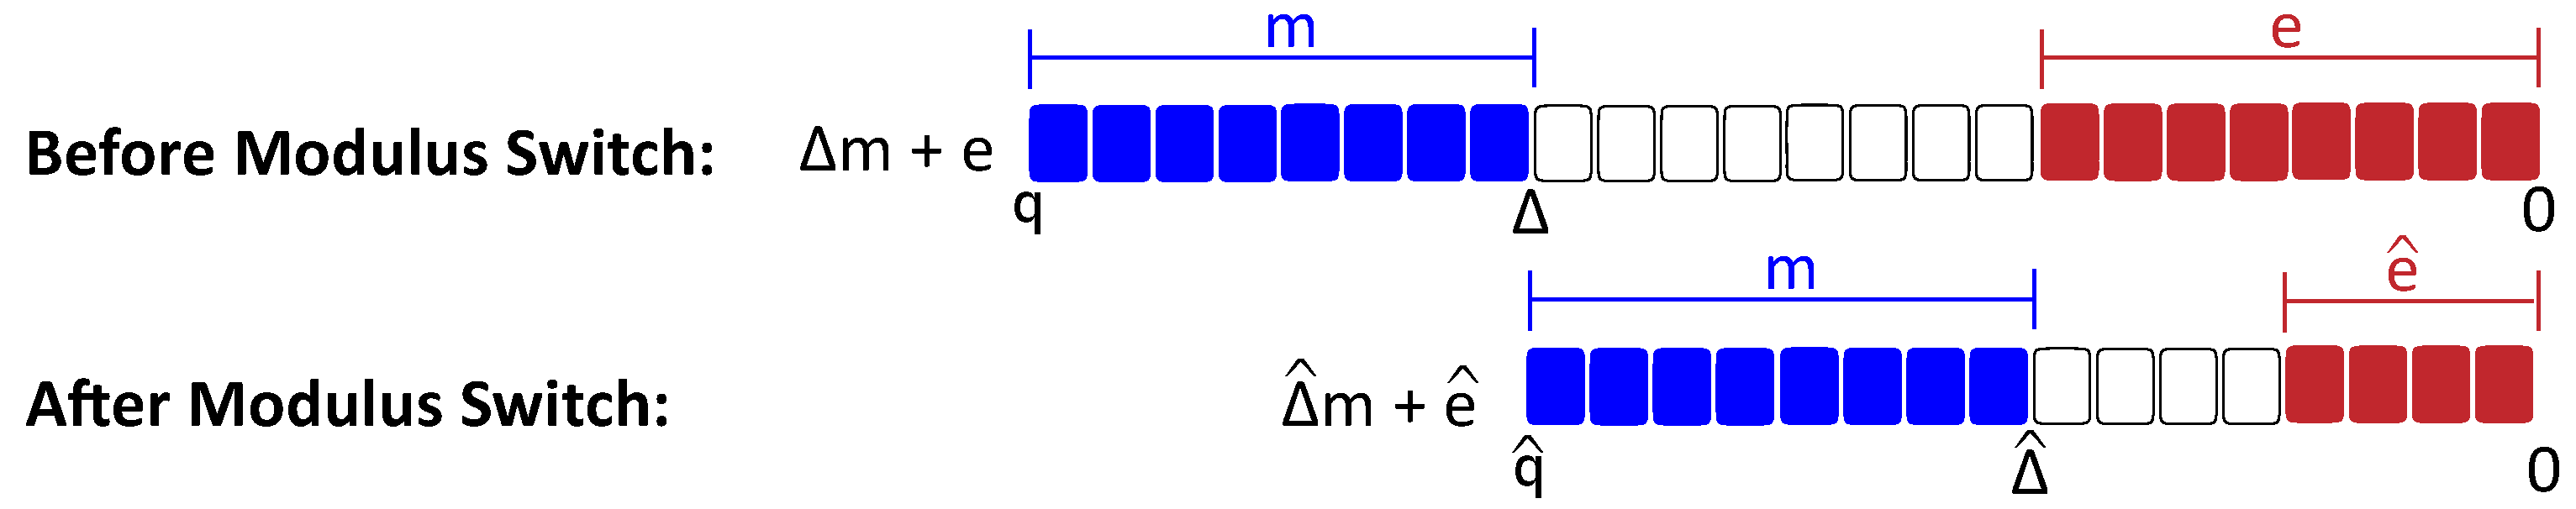
\includegraphics[width=0.7\linewidth]{figures/modulus-switching.pdf}
  \caption{An illustration of scaled plaintext with a noise: $\Delta \cdot m + e \in \mathbb{Z}_q$}
  \label{fig:modulus-switch}
\end{figure}

\para{Reduced Distance between $m$ and $e$:} After modulus switching of an LWE ciphertext from $q \rightarrow \hat{q}$, the underlying plaintext (containing a noise) $\Delta m + e$ gets shrunk to $\hat{\Delta}m + \hat{e}$, as illustrated in \autoref{fig:modulus-switch}. Note that after the modulus switch from $q \rightarrow \hat{q}$, $\Delta m$ is down-scaled to $\hat{\Delta} m$ without losing its bit data. Notably, the plaintext value $m$ stays the same after the modulus switch, while its scaling factor $\Delta$ gets reduced to $\hat{\Delta}$ and the noise $e$ gets reduced to $\hat e$. However, after the modulus switch, the distance between $\hat e$'s MSB and $\hat \Delta m$'s LSB gets reduced compared to the distance between $e$'s MSB and $\Delta m$'s LSB.




%\para{Hard Threshold on the $\Delta m$ Term's Value:} In \autoref{subsubsec:glwe-add-cipher-discuss}, we explained that the value of $\Delta m$ should not overflow or underflow its MSB $q$ during homomorphic computation (i.e., $\Delta m$ should be within the range of modulo $q$ without wrapping around), because if it wraps around the MSB, then our derived congruence relation of modulus switch loses its correctness. This is necessary in order to get the correct functionality of modulus switch on LWE ciphertexts. In particular, if we need to handle the case of $\Delta m$'s overflow, then our congruence relation of modulus switch should include the additional term $H_2 \cdot \Delta$ to take into account the added multiples of $\Delta$ caused by the overflows of $\Delta m$. But problematically, this term does not get eliminated during the modulus switch as $H_2 \cdot \Delta$ is not divisible by $\hat{q}$, which breaks our derived congruence relation above. Therefore, the applications of GLWE homomorphic encryption should ensure to manage their scaled plaintext $\Delta m$ to be always within than its maximum upper and minimum lower boundaries of the ciphertext modulus domain (i.e., $[0, q - 1]$ or $[-\dfrac{q}{2}, \dfrac{q}{2} - 1]$) throughout all computations. Meanwhile, the masking terms $A_i\cdot S_i$ are allowed to overflow or underflow ciphertext indefinitely during homomorphic computations, because during the decryption procedure they will be exactly subtracted and become zeroed out modulo $q$.  


\subsection{RLWE Modulus Switching}
\label{subsec:modulus-switch-rlwe}




RLWE modulus switching is similar to LWE modulus switching. Recall that the RLWE cryptosystem (\autoref{subsec:rlwe-enc}) comprises the following components:

\begin{itemize}
\item \textbf{\underline{Setup}: } 
$\Delta = \dfrac{q}{t}$, \text{ } $S = s_0 + s_1X + s_2X^2 + \cdots + s_{n-1}X^{n-1} \xleftarrow{\$} \mathcal{R}_{\langle n, 2 \rangle}$

$ $

\item \textbf{\underline{Encryption Input}: } 

$M \in \mathcal{R}_{\langle n, t \rangle}$

$A = a_0 + a_1X + a_2X^2 + \cdots + a_{n-1}X^{n-1} \xleftarrow{\$} \mathcal{R}_{\langle n, q \rangle}$

$E = e_0 + e_1X + e_2X^2 + \cdots + e_{n-1}X^{n-1} \xleftarrow{\chi_\sigma} \mathcal{R}_{\langle n, q \rangle}$ 

$ $

\item \textbf{\underline{Encryption}: } 
$\textsf{RLWE}_{S,\sigma}(\Delta \cdot M) = (A, B) \in \mathcal{R}_{\langle n,q \rangle}^2$ 

, where $B = A \cdot S + \Delta \cdot M + E = b_0 + b_1X + b_2X^2 + \cdots + b_{n-1}X^{n-1}$

$ $

\item \textbf{\underline{Decryption}: } $\textsf{RLWE}^{-1}_{S,\sigma}(C) = B - A \cdot S = \Delta  M + E \text{ } \in \mathcal{R}_{\langle n,q \rangle}$ 
\end{itemize}

$ $

RLWE modulus switching is done as follows:

\begin{tcolorbox}[title={\textbf{\tboxlabel{\ref*{subsec:modulus-switch-rlwe}} RLWE Modulus Switching}}]

For an RLWE ciphertext $(A, B)$ where $B = AS + \Delta M + E$ and $M \in \mathcal{R}_{\langle n, q \rangle}$, modulus switch of the ciphertext from $q$ to $\hat q$ is equivalent to updating $(A, B)$ to $(\hat A, \hat B)$ as follows:


$\hat{A} = \hat{a}_0 + \hat{a}_1X + \hat{a}_2X^2 + \cdots + \hat{a}_{n-1}X^{n-1}$, where each $\hat{a}_i = \Big\lceil a_i\dfrac{\hat{q}}{q} \Big\rfloor \in \mathbb{Z}_{\hat{q}}$ 

$\hat{B} = \hat{b}_0 + \hat{b}_1X + \hat{b}_2X^2 + \cdots + \hat{b}_{n-1}X^{n-1}$, where each $\hat{b}_i = \Big\lceil b_i\dfrac{\hat{q}}{q} \Big\rfloor \in \mathbb{Z}_{\hat{q}}$

$\textsf{RLWE}_{{S},\sigma}(\hat{\Delta}  M) = (\hat{A}, \hat{B}) \in \mathcal{R}_{\langle n, \hat{q} \rangle}^{2}$ 

$ $

The above update effectively changes $\Delta$ and $E$ as follows:

$\hat{\Delta} = \Delta\dfrac{\hat{q}}{q}$ \textcolor{red}{\# which should be an integer}

$\hat{E} = \hat{e}_0 + \hat{e}_1X + \hat{e}_2X^2 + \cdots + \hat{e}_{n-1}X^{n-1}$, where each $\hat{e}_i = \Big\lceil e_i\dfrac{\hat{q}}{q} \Big\rfloor \in \mathbb{Z}_{\hat{q}}$

$ $

Meanwhile, $S$ and $M$ stay the same as before.

\end{tcolorbox}

The proof is similar to that of LWE modulus switching.

$ $

\textbf{\underline{Proof}}

\begin{enumerate}
\item Note the following: 

$\hat{b}_i = \Big\lceil b_i \dfrac{\hat{q}}{q} \Big\rfloor = b_i\dfrac{\hat{q}}{q} + \epsilon_{b_i}$ (where $-0.5 < \epsilon_{b_i} < 0.5$, a rounding drift error)

$\hat{a}_i = \Big\lceil a_i \dfrac{\hat{q}}{q} \Big\rfloor = a_i\dfrac{\hat{q}}{q} + \epsilon_{a_i}$ (where $-0.5 < \epsilon_{a_i} < 0.5$)

$\hat{e}_i = \Big\lceil e_i \dfrac{\hat{q}}{q} \Big\rfloor = e_i\dfrac{\hat{q}}{q} + \epsilon_{e_i}$ (where $-0.5 < \epsilon_{e_i} < 0.5$)

\item Note the following: 


$B - A\cdot S$ 

$ = (b_0 + b_1X + \gap{$\cdots$} + b_{n-1}X^{n-1} ) - (a_{0} + a_{1}X + \gap{$\cdots$} + a_{n-1}X^{n-1})(s_{0} + s_{1}X + \gap{$\cdots$} + s_{n-1}X^{n-1})$ 


$ = \left(b_0 - \left( \sum\limits_{i=0}^{0}(a_{0-i}s_{i}) - \sum\limits_{i=1}^{n-1}(a_{n-i}s_{i}) \right)\right)$

$ + \left(b_1 - \left( \sum\limits_{i=0}^{1}(a_{1-i}s_{i}) - \sum\limits_{i=2}^{n-1}(a_{n+1-i}s_{i})   \right) \right)\cdot X$ 



$ + \left(b_2 - \left( \sum\limits_{i=0}^{2}(a_{2-i}s_{i}) - \sum\limits_{i=3}^{n-1}(a_{n+2-i}s_{i})   \right) \right)\cdot X^2$ 


$\gap{$\vdots$}$ 


$ + \left(b_{n-1} - \left(  \sum\limits_{i=0}^{n-1}(a_{n-1-i}s_{i}) -  \sum\limits_{i=n}^{n-1}(a_{n+n-1-i}s_{i})  \right) \right)\cdot X^{n-1}$ \textcolor{red}{\# Grouping the terms by same exponents}

$ $

$= \sum\limits_{h=0}^{n-1}  \left(b_h - \left( \sum\limits_{i=0}^{h}(a_{h-i}s_{i}) -  \sum\limits_{i=h+1}^{n-1}(a_{n+h-i}s_{i})  \right) \right)\cdot X^{h}  $

%$ $
$ $

Thus,

$ $

$B = \sum\limits_{h=0}^{n-1}  b_h  X^{h}  $

$A\cdot S = \sum\limits_{h=0}^{n-1}  \left(\sum\limits_{i=0}^{h}(a_{h-i}s_{i}) - \sum\limits_{i=h+1}^{n-1}(a_{n+h-i}s_{i}) \right)\cdot X^{h}  $

%$= \sum\limits_{h=0}^{n-1}  C_h \cdot X^{h}  $, where $C_h = b_h - \left(  \sum\limits_{i=0}^{h}(a_{h-i}s_{i}) - \sum\limits_{i=h+1}^{n-1}(a_{n+h-i}s_{i})  \right)$

$ $




\item Based on step 2,

$B = A \cdot S + \Delta  M + E$ 


$\sum\limits_{h=0}^{n-1}  b_h  X^{h}  = \sum\limits_{h=0}^{n-1}  \left(\sum\limits_{i=0}^{h}(a_{h-i}s_{i}) - \sum\limits_{i=h+1}^{n-1}(a_{n+h-i}s_{i}) \right)\cdot X^{h}  + \Delta \sum\limits_{h=0}^{n-1}  m_h  X^{h} + \sum\limits_{h=0}^{n-1}  e_h  X^{h}  \in \mathbb{Z}_q$

$\sum\limits_{h=0}^{n-1}  b_h  X^{h}  = \sum\limits_{h=0}^{n-1}  \left(\sum\limits_{i=0}^{h}(a_{h-i}s_{i}) - \sum\limits_{i=h+1}^{n-1}(a_{n+h-i}s_{i}) \right)\cdot X^{h}  + \Delta \sum\limits_{h=0}^{n-1}  m_h  X^{h} + \sum\limits_{h=0}^{n-1}  e_h  X^{h} + H \cdot q$

(where modulo $q$ is replaced by adding $H \cdot q$, an $(n-1)$-degree polynomial whose each coefficient $c_i$ is some multiple of $q$)

$ $

\item According to step 1 and 3, for each $j$ in $0 \leq j \leq n-1$:

$\hat{b}_j = b_j\dfrac{\hat{q}}{q} + \epsilon_{b_j} \in \mathbb{Z}_{\hat{q}}$

$= \left(\sum\limits_{i=0}^{j}(a_{j-i}s_{i}) - \sum\limits_{i=j+1}^{n-1}(a_{n+j-i}s_{i}) + \Delta m_j + e_j + c_j \cdot q\right) \cdot \dfrac{\hat{q}}{q} + \epsilon_{b_j}$

$= \dfrac{\hat{q}}{q} \sum\limits_{i=0}^{j}(a_{j-i}s_{i}) - \dfrac{\hat{q}}{q} \sum\limits_{i=j+1}^{n-1}(a_{n+j-i}s_{i}) + \dfrac{\hat{q}}{q} \cdot \Delta m_j + \dfrac{\hat{q}}{q} e_j + \dfrac{\hat{q}}{q} \cdot c_j \cdot q + \epsilon_{b_j}$

$=  \sum\limits_{i=0}^{j}\left(\dfrac{\hat{q}}{q}\cdot a_{j-i}s_{i}\right) - \sum\limits_{i=j+1}^{n-1}\left(\dfrac{\hat{q}}{q} \cdot a_{n+j-i}s_{i}\right) + \hat{\Delta} m_j + (\hat{e}_j - \epsilon_{e_j}) + \hat{q} \cdot c_j + \epsilon_{b_j}$

$=  \sum\limits_{i=0}^{j}((\hat{a}_{j-i}-\epsilon_{a_{j-i}})\cdot s_{i}) - \sum\limits_{i=j+1}^{n-1}((\hat{a}_{n+j-i}-\epsilon_{a_{n+j-i}})\cdot s_{i}) + \hat{\Delta} m_j + (\hat{e}_j - \epsilon_{e_j}) + \hat{q} \cdot c_j + \epsilon_{b_j}$

$=  \sum\limits_{i=0}^{j}(\hat{a}_{j-i}s_i) 
- \sum\limits_{i=j+1}^{n-1}(\hat{a}_{n+j-i}s_i)
- \sum\limits_{i=0}^{j}(\epsilon_{a_{j-i}} s_i)
+ \sum\limits_{i=j+1}^{n-1}(\epsilon_{a_{n+j-i}} s_i)
+ \hat{\Delta} m_j + (\hat{e}_j - \epsilon_{e_j}) + \hat{q} \cdot c_j + \epsilon_{b_j}$


$=  \left(\sum\limits_{i=0}^{j}(\hat{a}_{j-i}s_i) 
- \sum\limits_{i=j+1}^{n-1}(\hat{a}_{n+j-i}s_i)\right)
+ \hat{\Delta} m_j + \hat{e}_j 
+ \left(\epsilon_{b_j} - \epsilon_{e_j}
- \sum\limits_{i=0}^{j}(\epsilon_{a_{j-i}} s_i)
+ \sum\limits_{i=j+1}^{n-1}(\epsilon_{a_{n+j-i}} s_i)\right) + \hat{q} \cdot c_j
$

$=  \left(\sum\limits_{i=0}^{j}(\hat{a}_{j-i}s_i) 
- \sum\limits_{i=j+1}^{n-1}(\hat{a}_{n+j-i}s_i)\right)
+ \hat{\Delta} m_j + \hat{e}_j 
+ \epsilon_{all} \in \mathbb{Z}_{\hat{q}}
$

\textcolor{red}{ \# where $\epsilon_{all} = \epsilon_{b_j} - \epsilon_{e_j}
- \sum\limits_{i=0}^{j}(\epsilon_{a_{j-i}} s_i)
+ \sum\limits_{i=j+1}^{n-1}(\epsilon_{a_{n+j-i}} s_i) \approx 0$}


$ $

\item To summarize, for each $0 \leq j \leq n-1 $, each polynomial degree coefficient $\hat{b_j}$ is approximately as follows:

$\hat{b}_j =  \left(\sum\limits_{i=0}^{j}(\hat{a}_{j-i}s_i) 
- \sum\limits_{i=j+1}^{n-1}(\hat{a}_{n+j-i}s_i)\right)
+ \hat{\Delta} m_j + \hat{e}_j 
+ \epsilon_{all}$

$ \approx \left(\sum\limits_{i=0}^{j}(\hat{a}_{j-i}s_i) 
- \sum\limits_{i=j+1}^{n-1}(\hat{a}_{n+j-i}s_i)\right)
+ \hat{\Delta} m_j + \hat{e}_j$

Thus, $(\hat{a}_0, \hat{a}_1, \gap{$\cdots$}, \hat{b}) = \textsf{RLWE}_{{S},\sigma}(\hat{\Delta}  M)$, decrypting which will give us $M$.

\begin{flushright}
\qedsymbol{} 
\end{flushright}

\end{enumerate}




\subsection{GLWE Modulus Switching}
\label{subsec:modulus-switch-glwe}

GLWE modulus switching is an extension of RLWE modulus switching. The only difference is that while RLWE's $A$ and $S$ are a single polynomial each, GLWE's $A$ and $S$ are a list of $k$ polynomials each. Thus, the same modulus switching technique as RLWE can be applied to GLWE for its $k$ polynomials.  

Recall that the GLWE cryptosystem (\autoref{subsec:glwe-enc}) is comprised of the following components:

\begin{itemize}
\item \textbf{\underline{Initial Setup}: } $\Delta = \dfrac{q}{t}$, \text{ } $\{S_i\}_{i=0}^{k-1} \xleftarrow{\$} \mathcal{R}_{\langle n, 2 \rangle}^k$

$ $

\item \textbf{\underline{Encryption Input}: } $M \in \mathcal{R}_{\langle n, t \rangle}$, \text{ } $\{A_i\}_{i=0}^{k-1} \xleftarrow{\$} \mathcal{R}_{\langle n,q \rangle}^{k}$, \text{ } $E \xleftarrow{\chi_\sigma} \mathcal{R}_{\langle n,q \rangle}$

$ $

\item \textbf{\underline{Encryption}: } $\textsf{GLWE}_{S,\sigma}(\Delta M) = (\{A_i\}_{i=0}^{k-1}, B) \text{ } \in \mathcal{R}_{\langle n,q \rangle}^{k + 1}$ 

, where $B = \sum\limits_{i=0}^{k-1}{(A_i \cdot S_i)} + \Delta  M + E \text{ } \in \mathcal{R}_{\langle n,q \rangle}$

$ $

\item \textbf{\underline{Decryption}: } $\textsf{GLWE}^{-1}_{S,\sigma}(C) = B - \sum\limits_{i=0}^{k-1}{(A_i \cdot S_i)} = \Delta  M + E \text{ } \in \mathcal{R}_{\langle n,q \rangle}$

\end{itemize}

$ $

GLWE modulus switching is done as follows:

\begin{tcolorbox}[title={\textbf{\tboxlabel{\ref*{subsec:modulus-switch-glwe}} GLWE Modulus Switching}}]

Given a GLWE ciphertext $(\vec A, B)$ where $B = \vec A\cdot \vec S + \Delta M + E \bmod q$ and $M \in \mathbb{R}_{\langle n, q \rangle}$, the modulus switch of the ciphertext from $q$ to $\hat q$ is equivalent to updating $(\vec A, B)$ to $(\hat{\vec A}, \hat B)$ as follows:


$\hat{A_i} = \hat{a}_{i,0} + \hat{a}_{i,1}X + \hat{a}_{i,2}X^2 + \cdots + \hat{a}_{i, {n-1}}X^{n-1}$, where each $\hat{a}_{i,j} = \Big\lceil a_{i,j}\dfrac{\hat{q}}{q} \Big\rfloor \in \mathbb{Z}_{\hat{q}}$ 


$\hat{B} = \hat{b}_0 + \hat{b}_1X + \hat{b}_2X^2 + \cdots + \hat{b}_{n-1}X^{n-1}$, where each $\hat{b}_j = \Big\lceil b_j\dfrac{\hat{q}}{q} \Big\rfloor \in \mathbb{Z}_{\hat{q}}$

$\textsf{GLWE}_{{S},\sigma}(\hat{\Delta}  M) = (\hat{A}, \hat{B}) \in \mathcal{R}_{\langle n, \hat{q} \rangle}^{k+1}$ 

$ $

The above update effectively changes $E$ and $\Delta$ as follows:

$\hat{E} = \hat{e}_0 + \hat{e}_1X + \hat{e}_2X^2 + \cdots + \hat{e}_{n-1}X^{n-1}$, where each $\hat{e}_j = \Big\lceil e_j\dfrac{\hat{q}}{q} \Big\rfloor \in \mathbb{Z}_{\hat{q}}$


$\hat{\Delta} = \Delta\dfrac{\hat{q}}{q}$ \textcolor{red}{\# which should be an integer}

$ $


Meanwhile, $\vec{S}$ and $M$ stay the same as before.



\end{tcolorbox}

The proof is similar to that of RLWE modulus switching. The modulus-switched GLWE ciphertext's culminating rounding drift error for each $j$-th polynomial coefficient in its congruence relationship (i.e., $B = \sum\limits_{i=0}^{k-1}A_i\cdot S_i + \Delta M + E$) is as follows:

$\epsilon_{j, all} = \epsilon_{b_j} - \epsilon_{e_j}
- \sum\limits_{l=0}^{k-1}\sum\limits_{i=0}^{j}(\epsilon_{a_{l,j-i}} \cdot s_{l,i})
+ \sum\limits_{l=0}^{k-1}\sum\limits_{i=j+1}^{n-1}(\epsilon_{a_{l,n+j-i}} \cdot s_{l,i})$

\textcolor{red}{ \# derived from the proof step 4 of Summary~\ref*{subsec:modulus-switch-rlwe}: $\epsilon_{all} = \epsilon_{b_j} - \epsilon_{e_j}
- \sum\limits_{i=0}^{j}(\epsilon_{a_{j-i}} s_i)
+ \sum\limits_{i=j+1}^{n-1}(\epsilon_{a_{n+j-i}} s_i)$}

$ $

Note that GLWE's modulus switching can have a bigger rounding drift error (about $k$ times) than that of RLWE's modulus switching. However, in the long run, they can cancel out and converge to 0 as they are sampled from the $\sigma$ distribution.